\documentclass[]{article}
\usepackage[T1]{fontenc}
\usepackage{lmodern}
\usepackage{amssymb,amsmath}
\usepackage{ifxetex,ifluatex}
\usepackage{fixltx2e} % provides \textsubscript
% use microtype if available
\IfFileExists{microtype.sty}{\usepackage{microtype}}{}
% use upquote if available, for straight quotes in verbatim environments
\IfFileExists{upquote.sty}{\usepackage{upquote}}{}
\ifnum 0\ifxetex 1\fi\ifluatex 1\fi=0 % if pdftex
  \usepackage[utf8]{inputenc}
\else % if luatex or xelatex
  \usepackage{fontspec}
  \ifxetex
    \usepackage{xltxtra,xunicode}
  \fi
  \defaultfontfeatures{Mapping=tex-text,Scale=MatchLowercase}
  \newcommand{\euro}{€}
\fi
\usepackage{color}
\usepackage{fancyvrb}
\DefineShortVerb[commandchars=\\\{\}]{\|}
\DefineVerbatimEnvironment{Highlighting}{Verbatim}{commandchars=\\\{\}}
% Add ',fontsize=\small' for more characters per line
\newenvironment{Shaded}{}{}
\newcommand{\KeywordTok}[1]{\textcolor[rgb]{0.00,0.44,0.13}{\textbf{{#1}}}}
\newcommand{\DataTypeTok}[1]{\textcolor[rgb]{0.56,0.13,0.00}{{#1}}}
\newcommand{\DecValTok}[1]{\textcolor[rgb]{0.25,0.63,0.44}{{#1}}}
\newcommand{\BaseNTok}[1]{\textcolor[rgb]{0.25,0.63,0.44}{{#1}}}
\newcommand{\FloatTok}[1]{\textcolor[rgb]{0.25,0.63,0.44}{{#1}}}
\newcommand{\CharTok}[1]{\textcolor[rgb]{0.25,0.44,0.63}{{#1}}}
\newcommand{\StringTok}[1]{\textcolor[rgb]{0.25,0.44,0.63}{{#1}}}
\newcommand{\CommentTok}[1]{\textcolor[rgb]{0.38,0.63,0.69}{\textit{{#1}}}}
\newcommand{\OtherTok}[1]{\textcolor[rgb]{0.00,0.44,0.13}{{#1}}}
\newcommand{\AlertTok}[1]{\textcolor[rgb]{1.00,0.00,0.00}{\textbf{{#1}}}}
\newcommand{\FunctionTok}[1]{\textcolor[rgb]{0.02,0.16,0.49}{{#1}}}
\newcommand{\RegionMarkerTok}[1]{{#1}}
\newcommand{\ErrorTok}[1]{\textcolor[rgb]{1.00,0.00,0.00}{\textbf{{#1}}}}
\newcommand{\NormalTok}[1]{{#1}}
\usepackage{graphicx}
% We will generate all images so they have a width \maxwidth. This means
% that they will get their normal width if they fit onto the page, but
% are scaled down if they would overflow the margins.
\makeatletter
\def\maxwidth{\ifdim\Gin@nat@width>\linewidth\linewidth
\else\Gin@nat@width\fi}
\makeatother
\let\Oldincludegraphics\includegraphics
\renewcommand{\includegraphics}[1]{\Oldincludegraphics[width=\maxwidth]{#1}}
\ifxetex
  \usepackage[setpagesize=false, % page size defined by xetex
              unicode=false, % unicode breaks when used with xetex
              xetex]{hyperref}
\else
  \usepackage[unicode=true]{hyperref}
\fi
\hypersetup{breaklinks=true,
            bookmarks=true,
            pdfauthor={},
            pdftitle={},
            colorlinks=true,
            urlcolor=blue,
            linkcolor=magenta,
            pdfborder={0 0 0}}
\urlstyle{same}  % don't use monospace font for urls
\setlength{\parindent}{0pt}
\setlength{\parskip}{6pt plus 2pt minus 1pt}
\setlength{\emergencystretch}{3em}  % prevent overfull lines
\setcounter{secnumdepth}{0}

\author{}
\date{}

\begin{document}

\subsection{Abstract}

We face a deluge of data that scientists need to deal with in many
different domains today. While there are already good solutions to some
parts of the data life cycle the applicability of the solutions to
certain scientific domains often varies. Especially research domains
with high degree of interdisciplinary interactions and heterogeneity in
methods and data in general like ecology face problems in dealing with
some valuable concepts like ontologies that potentially can be used to
improve or automate some of the most common tasks in analyses like
finding relevant data, cleaning and merging of datasets. We here
introduce the \texttt{rbefata} package that connects to the open source
data management platform \texttt{BEFdata} that has been developed and is
used within the BEF-China experiment. We show the use of the package in
combination with the portal using an example workflow that integrates
three datasets from the BEF-China experiment representing an analysis
that has been published already. We discuss the combination of the R
package \texttt{rbefdata} and the data poral in the context of state of
the art data management as well as we give an outlook on upcoming
features that will bring semantical featues like smart merges based on
an ontology we created.

\subsection{Introduction}

With a growing awareness on the long term value of data, much effort has
been put into building data management platforms, to preserve all kind
of environmental and historic data, over the last years (e.g.~diversity
workbench, BEFdata). Many specialized solutions for different scientific
disciplines appeared that provide data management plans for small scale
projects or collaborations as well as for large data producing long term
or remote sensing projects. An ongoing trend in that context is the
development of integrative databases or data portals. They serve as
nodes that collect data from smaller databases of a certain domain and
they give researchers of that domain the opportunity to access a wide
range of relevant data from one place. This portals in fact offer a
solution to to one of the most pressing problems that we face with our
valuable data today, their lost.

Another big problem with data, especially in terms of reuse of available
data, is the general understanding of datasets. Usually plain datasets
say nothing, to one who is not familiar with it and they are even hard
to decipher by the author itself after some time has passed. It is
usually hard to remember exactly what methods have been used to collect
a certain columns data or what the abbreviations or headers in the
dataset mean. To solve this this problem metadata frameworks have been
developed and published as standards so nobody really needs to think
about an own set of requirements to describe its data. The Ecological
Metadata Language is only one example for that. While this theoretically
solves the problem with not well described datasets it is still hard to
make people use it extensively as this usually always means to learn new
tools that help with the description process (e.g morpho, data up).

While well described data helps a lot in understanding datasets and on
deciding upon the relevance and applicability in a certain analysis
there is still lots of manual intervention necessary after that to
prepare the data for analysis (cite yourself? or xxx). It may needs to
be cleaned, imputed, reshaped and merged which usually takes up to 70\%
of the analysis workflow, before the smart models can be applied to the
data to find interesting patters (cite the workflow paper of Karin and
me). This preparation steps not only are time and labour intensive but
also potentially error prone, especially as the complexity of analyses
grows.

Ontologies, formal representations of knowledge potentially offer a
sophisticated tool to deal with that step of data preparation (cite
supporting ecology as data intensive science). While they are already
used in some research domains like genetics (cite xxx), other domains
face more problems using it. For example in ecology, that has grown into
a very collaborative, interdisciplinary and data intensive science over
the last decade, to address questions on a greater temporal and spatial
scale (e.g michener et al 2012). The data here is mainly provided by
small scale studies spread all over the world (e.g heidorn2009 shedding
light on the dark) but also through bigger long term projects like LTER
(cite xxx), BEF-China (cite xxx), governmental projects and local
initiatives (cite xxx). This in fact results in a wild growing, complex
and heterogeneous data landscape in that we need to deal with. The
application of ontologies in ecology is discussed controversially (cite
xxx) which is mainly related to the heterogeneity of the research domain
and it is argued that they can be a benefit, but it is hard to set up a
sophisticated ontology covering all necessary terms and relation of a
that complex research domain like ecology.

As there is a growing demand to use and reuse available data and to
embed small heterogeneous data into a wider context in ecology we here
introduce the R package \texttt{rbefdata} that in combination with
BEFdata exactly deals with that. We showcase the functionality of the
package available with version 0.3.5 creating a workflow for integration
of three datasets and discuss the rbefdata package and BEFdata in the
light of future developments on the integration of ontologies that will
make finding data, smart merges and unit conversion possible to help
researchers to deal with the upcoming challenges in dealing with data
like integration of heterogeneous datasets.

\subsection{Material and Methods}

\subsubsection{BEF-China and the BEFdata portal}

The BEF-China experiment is a Biodiversity Ecosystem Functioning (BEF)
experiment funded by the German science foundation (DFG, FOR 891). It is
located in the subtropics of China in the provinces Jianxi and Zhejiang.
The BEF-China research group (www.bef-china.de) uses two main research
platforms. An experimental forest diversity gradient of
50\textasciitilde{}ha, and 27 observational plots of 30x30 m each
located in the Gutianshan Nature Reserve. The observational plots were
selected according to a crossed sampling design along tree species
richness and stand age. The data for the workflow on carbon pools stems
from 22 to 116 years consisting of 14 to 35 species (cite Bruelheide,
2010).

The \href{http://befdataproduction.biow.uni-leipzig.de/}{BEFdata} portal
is an open source data management platform developed within the
BEF-China project. It adheres to standards like the Ecological Metadata
Language for describing datasets with metadata and is specialized in
harmonizing small heterogeneous data that usually has to be dealt with
in BEF. But its specialization makes it also very valuable to use in any
other scientific domain that needs to deal with complex small and
heterogeneous data.

The portal offers a social component where researchers can shop datasets
and write a paper proposals based on the datasets in the shopping cart.
In the process of creating a proposal some information like a title, a
rationale, an envisaged journal and date needs to be provided. Sending
in a proposal a researcher asks for access to the datasets and provides
the data owners with necessary information about the paper. The data
owners then can decide if and how they like to participate in the
upcoming paper or if they only like to get acknowledged for providing
their data (cite Karin).

\subsubsection{The proposal}

We use an already published dataset as an example to present the
functionalities and interlinkages between the BEF China dataportal and
rbefdata. To test the effect of species richness on system N retention
and tree sapling N uptake we conducted a 15N tracer experiment in a
young tree plantation. To this end, saplings of four abundant early
successional tree species have been planted in monocultures, in two- and
four-species mixtures, and as individual trees. Afforestations are
increasing globally to produce timber and pulp wood, but also to enhance
ecosystem services such as carbon sequestration, nutrient retention, or
groundwater recharge. In order to further optimise these services with
regard to balanced nutrient (particularly nitrogen) cycles, it is
important to know whether the use of mixtures of native tree species in
afforestation projects promotes greater acquisition and retention of
nitrogen compared to the currently established large-scale monocultures.
Experimental design and data acquisition Four species were chosen for
the experiment: Schima superba Gardn. et Champ. and Elaeocarpus
decipiens Hemsley (evergreen), Quercus serrata Murray and Castanea
henryi (Skan) Rehd. et Wils. (deciduous; Yu et al. 2001). The following
planting schemes were established in 1-m² plots. In each plot 16
saplings were planted in an array of four by four. Monocultures,
two-species combinations and four-species combinations were established.
The four study species provided a total of eleven species combinations
four monocultures, six two-species combinations, and one four-species
combination. All treatments were replicated four times, once in each of
the four blocks. Pulse labelling with 15NH415NO3 (98\% 15N) was
performed in August and in September 2009. Leaf, fine root and soil
samples have been collected in September 2010. Samples have been
analysed for 15N content and leaf, fine root and soil recovery have been
calculated. The sum of the three compartement recoveries is referred to
as system N retention. Relative leaf, root and soil recovery was
calculted as percentage of system N retention (for a detailed
description of the material and methods we refer to Lang et al. 2013).

\begin{itemize}
\itemsep1pt\parskip0pt\parsep0pt
\item
  figure shows the proposal page
\end{itemize}

\begin{figure}[htbp]
\centering
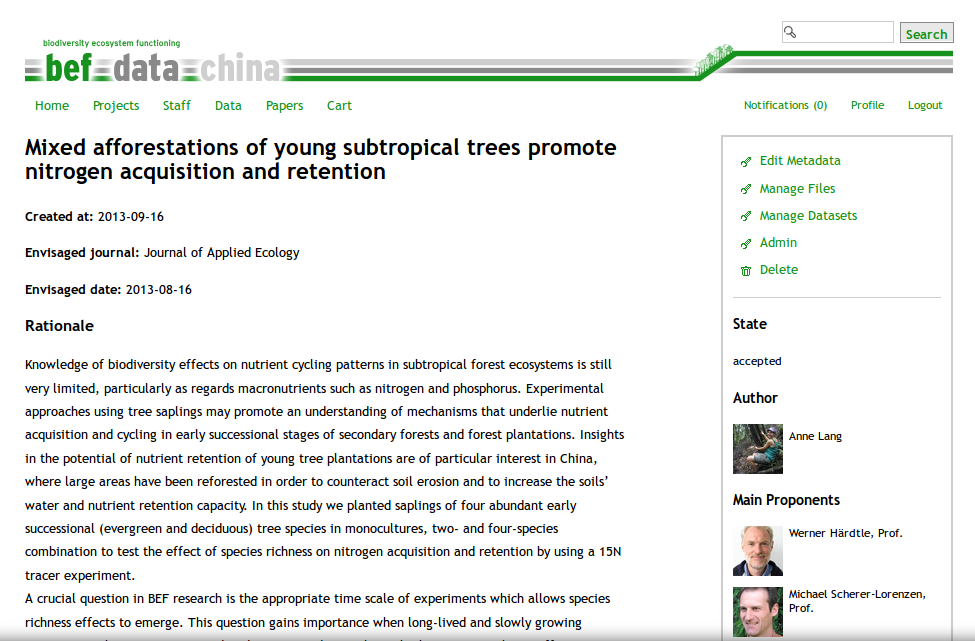
\includegraphics{./figure/static/showcase_proposal.png}
\caption{showcase\_proposal}
\end{figure}

\subsubsection{rbefdata}

The \texttt{rbefdata} package started its development within the
BEF-Cina experiment. Meanwhile it is part of the rOpenSci package
porfolio (http://ropensci.org/), which is a community driven approach to
wrap all science APIs and to create solutions to pull data from
different repositories into R for analysis.

The package can be installed from the CRAN package repository
(https://github.com/befdata/befdata) and enables access to the data,
meta data structures of the platform and provides convenient methods to
pull single or multiple dataset into the R environment in one step for
analysis.

Additionally it offers functions that help to upload final results
datasets with the script attached that has been used to derive the
results from the original datasets which provides a valuable insight
into data provenance and also is a stepping stone for reproducible
research.

\subsection{Usecase (results)}

The next step after the an accepted paper proposal is to setup the
\texttt{rbefdata} package. This requires loading the package and setting
the required package options. Having a look into the options list
reveals several fields that can be filled in, like the URL to the
BEFdata server, user credentials and a download folder name that is used
to store downloaded freeformat files. The tematres server related URLs
in the options are part of upcomming features that are non fully
functional on the time of writing.

The most essential setting for the workflow we present here is the user
credentials. These are used to authenticate the user against the portal
to ensure the access to the data has been granted and to log the data
access. Setting the URL is not required here as it defaults to the
BEF-China project instance of the BEFdata portal that we retrieve data
from. If one has set up an own instance of the BEFdata portal, this URL
needs to be changed so the package communicates with the right server
(see box below).

\begin{Shaded}
\begin{Highlighting}[]
\KeywordTok{require}\NormalTok{(rbefdata)}
\CommentTok{# options list}
\KeywordTok{bef.options}\NormalTok{()}
\end{Highlighting}
\end{Shaded}

\begin{verbatim}
## $url
## [1] "http://china.befdata.biow.uni-leipzig.de"
## 
## $tematres_url
## [1] "http://tematres.befdata.biow.uni-leipzig.de/vocab/index.php"
## 
## $tematres_service_url
## [1] "http://tematres.befdata.biow.uni-leipzig.de/vocab/services.php"
## 
## $download_dir
## [1] "downloads"
## 
## $user_credentials
## [1] ""
\end{verbatim}

\begin{Shaded}
\begin{Highlighting}[]

\CommentTok{# querry single options}
\KeywordTok{bef.options}\NormalTok{(}\StringTok{"url"}\NormalTok{)}
\end{Highlighting}
\end{Shaded}

\begin{verbatim}
## [1] "http://china.befdata.biow.uni-leipzig.de"
\end{verbatim}

\begin{Shaded}
\begin{Highlighting}[]
\CommentTok{# set credentials example}
\KeywordTok{bef.options}\NormalTok{(}\DataTypeTok{user_credentials =} \StringTok{"aölkjspoiul12"}\NormalTok{)}
\end{Highlighting}
\end{Shaded}

\begin{Shaded}
\begin{Highlighting}[]
\CommentTok{# set URL example}
\KeywordTok{bef.options}\NormalTok{(}\DataTypeTok{url =} \StringTok{"http://my.own.befdata.instance.com"}\NormalTok{)}
\end{Highlighting}
\end{Shaded}

After the setup of the \texttt{rbefdata} package we can start right away
using data from the proposal. A (proposal) download function is used for
that which draws all associated datasets of the proposal into the R
environment in one single step (see blow). The functin reuires the ID of
the proposal that can be found in the URL of the proposal on the BEFdata
portal (see blow).

\begin{verbatim}
# the id is 90
http://befdataproduction.biow.uni-leipzig.de/paperproposals/90
\end{verbatim}

\begin{Shaded}
\begin{Highlighting}[]
\CommentTok{# proposal id is}
\NormalTok{datasets = }\KeywordTok{bef.get.datasets_for_proposal}\NormalTok{(}\DataTypeTok{id =} \DecValTok{90}\NormalTok{)}
\NormalTok{extract_one_dataset = datasets[[}\DecValTok{1}\NormalTok{]]}
\end{Highlighting}
\end{Shaded}

\begin{itemize}
\itemsep1pt\parskip0pt\parsep0pt
\item
  Inspect datasets
\item
  after download (attributes())
\item
  in general bef.get.metadata\_for(dataset = id)
\end{itemize}

As the BEFdata portal provides metadata via EML standard, we also make
use of that within rbefdata. Each dataset on download is associated with
the metadata provided by its authors. This information can be extracted
using the built-in R function \texttt{attributes()} (see code box
below). As this requires granted access rights to the dataset, there is
also a function especially to only draw the metadata which is always
free for download.

\begin{Shaded}
\begin{Highlighting}[]
\CommentTok{# extract title of one dataset}
\KeywordTok{attributes}\NormalTok{(datasets[[}\DecValTok{1}\NormalTok{]])$title}
\end{Highlighting}
\end{Shaded}

\begin{verbatim}
## [1] "Competition of saplings for N -Pilot- system 15N retention"
\end{verbatim}

\begin{Shaded}
\begin{Highlighting}[]

\CommentTok{# for all dataset in the proposal}
\NormalTok{titles = }\KeywordTok{sapply}\NormalTok{(datasets, function(x) }\KeywordTok{attributes}\NormalTok{(x)$title)}
\NormalTok{titles}
\end{Highlighting}
\end{Shaded}

\begin{verbatim}
## [1] "Competition of saplings for N -Pilot- system 15N retention"           
## [2] "Plottreatment and -location within the blocks of the Pilot-Experiment"
\end{verbatim}

\begin{Shaded}
\begin{Highlighting}[]

\CommentTok{# other metadata available}
\KeywordTok{names}\NormalTok{(}\KeywordTok{attributes}\NormalTok{(datasets[[}\DecValTok{1}\NormalTok{]]))}
\end{Highlighting}
\end{Shaded}

\begin{verbatim}
##  [1] "names"                    "class"                   
##  [3] "row.names"                "title"                   
##  [5] "abstract"                 "publicationDate"         
##  [7] "language"                 "creators"                
##  [9] "authors"                  "intellectualRights"      
## [11] "distribution"             "keywords"                
## [13] "generalTaxonomicCoverage" "samplingDescription"     
## [15] "spatial_coverage"         "temporal_coverage"       
## [17] "related_material"         "columns"
\end{verbatim}

\begin{Shaded}
\begin{Highlighting}[]

\CommentTok{# only get metadtata by dataset id}
\KeywordTok{bef.portal.get.metadata}\NormalTok{(}\DataTypeTok{dataset =} \DecValTok{335}\NormalTok{)$title}
\end{Highlighting}
\end{Shaded}

\begin{verbatim}
## [1] "Competition of saplings for N -Pilot- system 15N retention"
\end{verbatim}

\begin{itemize}
\item
  both datasets contain a \texttt{plot\_id} that can be used for merge
\item
  extract into separate datasets
\item
  We need to merge them two by two.
\item
  to analyse the dataset of system N retention we do need information
  about species diversity of the plots and the information about which
  plot is placed in which block from the design dataset. Furthermore we
  need values of the initial basal diameter from the dataset Nrecov
\end{itemize}

\begin{Shaded}
\begin{Highlighting}[]
\CommentTok{# extract into separate datasets}
\NormalTok{Nretention = datasets[[}\DecValTok{1}\NormalTok{]]}
\NormalTok{design = datasets[[}\DecValTok{2}\NormalTok{]]}

\CommentTok{# overview about the contents of the datasets}
\KeywordTok{names}\NormalTok{(Nretention)}
\end{Highlighting}
\end{Shaded}

\begin{verbatim}
## [1] "plot_id"      "recov_plot"   "perleaf_plot" "perroot_plot"
## [5] "perbio_plot"  "persoil_plot" "gbd_T0.mm."
\end{verbatim}

\begin{Shaded}
\begin{Highlighting}[]
\KeywordTok{names}\NormalTok{(design)}
\end{Highlighting}
\end{Shaded}

\begin{verbatim}
##  [1] "block"                    "x"                       
##  [3] "y"                        "plot_id"                 
##  [5] "control_ID"               "block_community_code"    
##  [7] "community_number"         "species_mixture"         
##  [9] "species_diversity"        "species_pool"            
## [11] "species_code"             "research_group_colour"   
## [13] "control"                  "closed_canopy"           
## [15] "density"                  "Natives"                 
## [17] "depth"                    "harvest"                 
## [19] "fungicide"                "inoculation"             
## [21] "pesticide"                "native"                  
## [23] "genetic_diverstiy"        "seed_addition"           
## [25] "fertilizer"               "plot_treatment_connected"
## [27] "sp1"                      "sp2"                     
## [29] "sp3"                      "sp4"                     
## [31] "sp5"                      "sp7"                     
## [33] "sp8"                      "sp11"                    
## [35] "sp_connected"
\end{verbatim}

\begin{itemize}
\itemsep1pt\parskip0pt\parsep0pt
\item
  However, this synthesis dataset now includes many columns that we do
  not need. Thus they will be excluded in a synthesis dataset we create.
\end{itemize}

\begin{Shaded}
\begin{Highlighting}[]
\CommentTok{# the synthesis dataset}
\NormalTok{syndata = }\KeywordTok{merge}\NormalTok{(Nretention, design)}

\CommentTok{# overview about the content of the synthesis dataset}
\KeywordTok{names}\NormalTok{(syndata)}
\end{Highlighting}
\end{Shaded}

\begin{verbatim}
##  [1] "plot_id"                  "recov_plot"              
##  [3] "perleaf_plot"             "perroot_plot"            
##  [5] "perbio_plot"              "persoil_plot"            
##  [7] "gbd_T0.mm."               "block"                   
##  [9] "x"                        "y"                       
## [11] "control_ID"               "block_community_code"    
## [13] "community_number"         "species_mixture"         
## [15] "species_diversity"        "species_pool"            
## [17] "species_code"             "research_group_colour"   
## [19] "control"                  "closed_canopy"           
## [21] "density"                  "Natives"                 
## [23] "depth"                    "harvest"                 
## [25] "fungicide"                "inoculation"             
## [27] "pesticide"                "native"                  
## [29] "genetic_diverstiy"        "seed_addition"           
## [31] "fertilizer"               "plot_treatment_connected"
## [33] "sp1"                      "sp2"                     
## [35] "sp3"                      "sp4"                     
## [37] "sp5"                      "sp7"                     
## [39] "sp8"                      "sp11"                    
## [41] "sp_connected"
\end{verbatim}

\begin{Shaded}
\begin{Highlighting}[]
\NormalTok{syndata = syndata[-}\KeywordTok{c}\NormalTok{(}\DecValTok{9}\NormalTok{:}\DecValTok{14}\NormalTok{, }\DecValTok{16}\NormalTok{:}\DecValTok{41}\NormalTok{)]}
\KeywordTok{names}\NormalTok{(syndata)}
\end{Highlighting}
\end{Shaded}

\begin{verbatim}
## [1] "plot_id"           "recov_plot"        "perleaf_plot"     
## [4] "perroot_plot"      "perbio_plot"       "persoil_plot"     
## [7] "gbd_T0.mm."        "block"             "species_diversity"
\end{verbatim}

\begin{Shaded}
\begin{Highlighting}[]

\NormalTok{### check for data properties (keep?)}
\KeywordTok{str}\NormalTok{(syndata)}
\end{Highlighting}
\end{Shaded}

\begin{verbatim}
## 'data.frame':    42 obs. of  9 variables:
##  $ plot_id          : Factor w/ 42 levels "pilot1D01","pilot1D02",..: 1 2 3 4 5 6 7 8 9 10 ...
##  $ recov_plot       : num  15.64 13.03 20.29 9.6 8.35 ...
##  $ perleaf_plot     : num  2.92 5.52 1.06 4.19 15.1 ...
##  $ perroot_plot     : num  1.001 1.369 0.516 1.086 5.098 ...
##  $ perbio_plot      : num  3.92 6.89 1.57 2.03 17.96 ...
##  $ persoil_plot     : num  96.1 93.1 98.4 98 82 ...
##  $ gbd_T0.mm.       : num  NA 3.69 2.88 6 7 ...
##  $ block            : Factor w/ 8 levels "1","2","3","4",..: 1 1 1 1 1 1 1 1 1 2 ...
##  $ species_diversity: int  1 1 1 2 2 2 2 2 4 1 ...
\end{verbatim}

\begin{Shaded}
\begin{Highlighting}[]

\NormalTok{### we want to use 'species_diversity' as a factor}

\NormalTok{syndata$species_diversity = }\KeywordTok{as.factor}\NormalTok{(syndata$species_diversity)}
\KeywordTok{attach}\NormalTok{(syndata)}

\NormalTok{### check response variables for normality and transform}

\CommentTok{# qqnorm(recov_plot^.5) qqline(recov_plot^.5,lty=2)}
\NormalTok{syndata$recov_plot_t = syndata$recov_plot^}\FloatTok{0.5}

\CommentTok{# qqnorm(perleaf_plot^.5) qqline(perleaf_plot^.5,lty=2)}
\NormalTok{syndata$perleaf_plot_t = syndata$perleaf_plot^}\FloatTok{0.5}
\NormalTok{### All response variables have been square root transformed}

\NormalTok{syndata$perroot_plot_t = syndata$perroot_plot^}\FloatTok{0.5}
\NormalTok{syndata$perbio_plot_t = syndata$perbio_plot^}\FloatTok{0.5}
\NormalTok{syndata$persoil_plot_t = syndata$persoil_plot^}\FloatTok{0.5}

\NormalTok{### round response varibles}
\NormalTok{syndata$recov_plot_t = }\KeywordTok{round}\NormalTok{(syndata$recov_plot_t, }\DataTypeTok{digits =} \DecValTok{2}\NormalTok{)}
\NormalTok{syndata$perleaf_plot_t = }\KeywordTok{round}\NormalTok{(syndata$perleaf_plot_t, }\DataTypeTok{digits =} \DecValTok{2}\NormalTok{)}
\NormalTok{syndata$perroot_plot_t = }\KeywordTok{round}\NormalTok{(syndata$perroot_plot_t, }\DataTypeTok{digits =} \DecValTok{2}\NormalTok{)}
\NormalTok{syndata$persoil_plot_t = }\KeywordTok{round}\NormalTok{(syndata$persoil_plot_t, }\DataTypeTok{digits =} \DecValTok{2}\NormalTok{)}
\KeywordTok{attach}\NormalTok{(syndata)}
\end{Highlighting}
\end{Shaded}

\begin{verbatim}
## The following objects are masked from syndata (position 3):
## 
##     block, gbd_T0.mm., perbio_plot, perleaf_plot, perroot_plot,
##     persoil_plot, plot_id, recov_plot, species_diversity
\end{verbatim}

\begin{itemize}
\itemsep1pt\parskip0pt\parsep0pt
\item
  we want to analyse our data by linear mixed effects models. Since our
  plots are clumbed in space, we use block as random factor we will use
  the we will use the packages (nlme) for model analysis and (multcomp)
  for post-hoc comparisons
\end{itemize}

\begin{verbatim}
## Loading required package: mvtnorm Loading required package: survival
## Loading required package: splines Loading required package: MASS Loading
## required package: nnet
\end{verbatim}

\begin{Shaded}
\begin{Highlighting}[]
\NormalTok{#### Model one Overall recovery/N retention}

\NormalTok{model1 = }\KeywordTok{lme}\NormalTok{(recov_plot_t ~ gbd_T0.mm. + species_diversity, syndata, }\DataTypeTok{random =} \NormalTok{~}\DecValTok{1} \NormalTok{\textbar{} }
    \NormalTok{block, }\DataTypeTok{na.action =} \NormalTok{na.omit, }\DataTypeTok{method =} \StringTok{"REML"}\NormalTok{)}
\KeywordTok{anova}\NormalTok{(model1)}
\end{Highlighting}
\end{Shaded}

\begin{verbatim}
##                   numDF denDF F-value p-value
## (Intercept)           1    34   871.4  <.0001
## gbd_T0.mm.            1    34     7.5  0.0098
## species_diversity     2    34     2.9  0.0708
\end{verbatim}

\begin{Shaded}
\begin{Highlighting}[]
\KeywordTok{summary}\NormalTok{(}\KeywordTok{glht}\NormalTok{(model1, }\DataTypeTok{linfct =} \KeywordTok{mcp}\NormalTok{(}\DataTypeTok{species_diversity =} \StringTok{"Tukey"}\NormalTok{)))}
\end{Highlighting}
\end{Shaded}

\begin{verbatim}
## 
##   Simultaneous Tests for General Linear Hypotheses
## 
## Multiple Comparisons of Means: Tukey Contrasts
## 
## 
## Fit: lme.formula(fixed = recov_plot_t ~ gbd_T0.mm. + species_diversity, 
##     data = syndata, random = ~1 | block, method = "REML", na.action = na.omit)
## 
## Linear Hypotheses:
##            Estimate Std. Error z value Pr(>|z|)  
## 2 - 1 == 0   -0.378      0.251   -1.51    0.279  
## 4 - 1 == 0    0.479      0.420    1.14    0.480  
## 4 - 2 == 0    0.858      0.398    2.15    0.076 .
## ---
## Signif. codes:  0 '***' 0.001 '**' 0.01 '*' 0.05 '.' 0.1 ' ' 1
## (Adjusted p values reported -- single-step method)
\end{verbatim}

\begin{Shaded}
\begin{Highlighting}[]

\NormalTok{## To adjust for the unbalanced experimental design, Anova Type II (package}
\NormalTok{## “car” (Fox & Weisberg 2011)) was used to test for main effects}

\NormalTok{model1c = }\KeywordTok{Anova}\NormalTok{(model1, }\DataTypeTok{type =} \StringTok{"II"}\NormalTok{)}
\NormalTok{model1c}
\end{Highlighting}
\end{Shaded}

\begin{verbatim}
## Analysis of Deviance Table (Type II tests)
## 
## Response: recov_plot_t
##                   Chisq Df Pr(>Chisq)   
## gbd_T0.mm.         7.42  1     0.0065 **
## species_diversity  5.73  2     0.0570 . 
## ---
## Signif. codes:  0 '***' 0.001 '**' 0.01 '*' 0.05 '.' 0.1 ' ' 1
\end{verbatim}

\begin{Shaded}
\begin{Highlighting}[]

\CommentTok{# vizual check plot(model1,resid(.)~fitted(.))}
\CommentTok{# plot(model1,recov_plot_t~fitted(.))}

\NormalTok{#### Model2 percentage leaf recovery of plot recovery}

\NormalTok{model2 = }\KeywordTok{lme}\NormalTok{(perleaf_plot_t ~ species_diversity, syndata, }\DataTypeTok{random =} \NormalTok{~}\DecValTok{1} \NormalTok{\textbar{} block, }
    \DataTypeTok{method =} \StringTok{"REML"}\NormalTok{)}
\KeywordTok{anova}\NormalTok{(model2)}
\end{Highlighting}
\end{Shaded}

\begin{verbatim}
##                   numDF denDF F-value p-value
## (Intercept)           1    36  273.07  <.0001
## species_diversity     2    36    6.55  0.0037
\end{verbatim}

\begin{Shaded}
\begin{Highlighting}[]
\KeywordTok{summary}\NormalTok{(}\KeywordTok{glht}\NormalTok{(model2, }\DataTypeTok{linfct =} \KeywordTok{mcp}\NormalTok{(}\DataTypeTok{species_diversity =} \StringTok{"Tukey"}\NormalTok{)))}
\end{Highlighting}
\end{Shaded}

\begin{verbatim}
## 
##   Simultaneous Tests for General Linear Hypotheses
## 
## Multiple Comparisons of Means: Tukey Contrasts
## 
## 
## Fit: lme.formula(fixed = perleaf_plot_t ~ species_diversity, data = syndata, 
##     random = ~1 | block, method = "REML")
## 
## Linear Hypotheses:
##            Estimate Std. Error z value Pr(>|z|)    
## 2 - 1 == 0    1.052      0.293    3.59   <0.001 ***
## 4 - 1 == 0    0.865      0.497    1.74     0.18    
## 4 - 2 == 0   -0.187      0.479   -0.39     0.92    
## ---
## Signif. codes:  0 '***' 0.001 '**' 0.01 '*' 0.05 '.' 0.1 ' ' 1
## (Adjusted p values reported -- single-step method)
\end{verbatim}

\begin{Shaded}
\begin{Highlighting}[]
\KeywordTok{Anova}\NormalTok{(model2, }\DataTypeTok{type =} \StringTok{"II"}\NormalTok{)}
\end{Highlighting}
\end{Shaded}

\begin{verbatim}
## Analysis of Deviance Table (Type II tests)
## 
## Response: perleaf_plot_t
##                   Chisq Df Pr(>Chisq)   
## species_diversity  13.1  2     0.0014 **
## ---
## Signif. codes:  0 '***' 0.001 '**' 0.01 '*' 0.05 '.' 0.1 ' ' 1
\end{verbatim}

\begin{Shaded}
\begin{Highlighting}[]

\CommentTok{# vizual check plot(model2,resid(.)~fitted(.))}
\CommentTok{# plot(model2,perleaf_plot_t~fitted(.))}


\NormalTok{### Model3 percentage root recovery of overall recovery}

\NormalTok{model3 = }\KeywordTok{lme}\NormalTok{(perroot_plot_t ~ species_diversity, syndata, }\DataTypeTok{random =} \NormalTok{~}\DecValTok{1} \NormalTok{\textbar{} block, }
    \DataTypeTok{method =} \StringTok{"REML"}\NormalTok{)}
\KeywordTok{anova}\NormalTok{(model3)}
\end{Highlighting}
\end{Shaded}

\begin{verbatim}
##                   numDF denDF F-value p-value
## (Intercept)           1    36   373.7  <.0001
## species_diversity     2    36     7.1  0.0024
\end{verbatim}

\begin{Shaded}
\begin{Highlighting}[]
\KeywordTok{summary}\NormalTok{(}\KeywordTok{glht}\NormalTok{(model3, }\DataTypeTok{linfct =} \KeywordTok{mcp}\NormalTok{(}\DataTypeTok{species_diversity =} \StringTok{"Tukey"}\NormalTok{)))}
\end{Highlighting}
\end{Shaded}

\begin{verbatim}
## 
##   Simultaneous Tests for General Linear Hypotheses
## 
## Multiple Comparisons of Means: Tukey Contrasts
## 
## 
## Fit: lme.formula(fixed = perroot_plot_t ~ species_diversity, data = syndata, 
##     random = ~1 | block, method = "REML")
## 
## Linear Hypotheses:
##            Estimate Std. Error z value Pr(>|z|)   
## 2 - 1 == 0    0.600      0.170    3.53    0.001 **
## 4 - 1 == 0    0.731      0.289    2.53    0.029 * 
## 4 - 2 == 0    0.130      0.278    0.47    0.883   
## ---
## Signif. codes:  0 '***' 0.001 '**' 0.01 '*' 0.05 '.' 0.1 ' ' 1
## (Adjusted p values reported -- single-step method)
\end{verbatim}

\begin{Shaded}
\begin{Highlighting}[]
\KeywordTok{Anova}\NormalTok{(model3, }\DataTypeTok{type =} \StringTok{"II"}\NormalTok{)}
\end{Highlighting}
\end{Shaded}

\begin{verbatim}
## Analysis of Deviance Table (Type II tests)
## 
## Response: perroot_plot_t
##                   Chisq Df Pr(>Chisq)    
## species_diversity  14.3  2    0.00079 ***
## ---
## Signif. codes:  0 '***' 0.001 '**' 0.01 '*' 0.05 '.' 0.1 ' ' 1
\end{verbatim}

\begin{Shaded}
\begin{Highlighting}[]

\CommentTok{# vizual check plot(model3,resid(.)~fitted(.))}
\CommentTok{# plot(model3,perleaf_plot_t~fitted(.))}


\NormalTok{### Model 4 percentage soil recovery of overall recovery}

\NormalTok{model4 = }\KeywordTok{lme}\NormalTok{(persoil_plot_t ~ species_diversity, syndata, }\DataTypeTok{random =} \NormalTok{~}\DecValTok{1} \NormalTok{\textbar{} block, }
    \DataTypeTok{method =} \StringTok{"REML"}\NormalTok{)}
\KeywordTok{anova}\NormalTok{(model4)}
\end{Highlighting}
\end{Shaded}

\begin{verbatim}
##                   numDF denDF F-value p-value
## (Intercept)           1    36   26200  <.0001
## species_diversity     2    36       4  0.0274
\end{verbatim}

\begin{Shaded}
\begin{Highlighting}[]
\KeywordTok{summary}\NormalTok{(}\KeywordTok{glht}\NormalTok{(model4, }\DataTypeTok{linfct =} \KeywordTok{mcp}\NormalTok{(}\DataTypeTok{species_diversity =} \StringTok{"Tukey"}\NormalTok{)))}
\end{Highlighting}
\end{Shaded}

\begin{verbatim}
## 
##   Simultaneous Tests for General Linear Hypotheses
## 
## Multiple Comparisons of Means: Tukey Contrasts
## 
## 
## Fit: lme.formula(fixed = persoil_plot_t ~ species_diversity, data = syndata, 
##     random = ~1 | block, method = "REML")
## 
## Linear Hypotheses:
##            Estimate Std. Error z value Pr(>|z|)  
## 2 - 1 == 0   -0.294      0.127   -2.32    0.050 .
## 4 - 1 == 0   -0.501      0.215   -2.33    0.049 *
## 4 - 2 == 0   -0.207      0.207   -1.00    0.570  
## ---
## Signif. codes:  0 '***' 0.001 '**' 0.01 '*' 0.05 '.' 0.1 ' ' 1
## (Adjusted p values reported -- single-step method)
\end{verbatim}

\begin{Shaded}
\begin{Highlighting}[]
\KeywordTok{Anova}\NormalTok{(model4, }\DataTypeTok{type =} \StringTok{"II"}\NormalTok{)}
\end{Highlighting}
\end{Shaded}

\begin{verbatim}
## Analysis of Deviance Table (Type II tests)
## 
## Response: persoil_plot_t
##                   Chisq Df Pr(>Chisq)  
## species_diversity  7.96  2      0.019 *
## ---
## Signif. codes:  0 '***' 0.001 '**' 0.01 '*' 0.05 '.' 0.1 ' ' 1
\end{verbatim}

\begin{Shaded}
\begin{Highlighting}[]

\CommentTok{# vizual check plot(model4,resid(.)~fitted(.))}
\CommentTok{# plot(model4,perleaf_plot_t~fitted(.))}
\end{Highlighting}
\end{Shaded}

\begin{figure}[htbp]
\centering
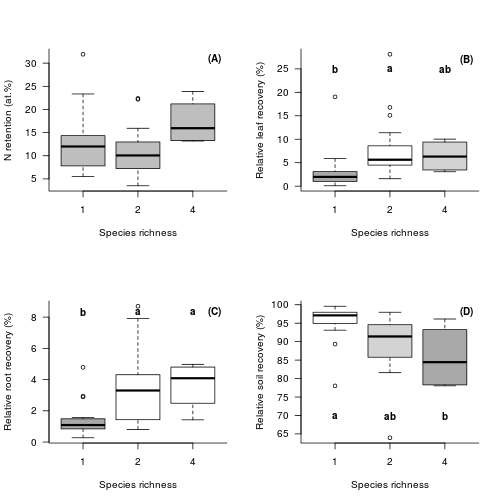
\includegraphics{figure/final_plot.png}
\caption{plot of chunk final\_plot}
\end{figure}

\subsection{Discussion}

\begin{itemize}
\item
  General discussion
\item
  high need to effective use/reuse data
\item
  relevant data needs to be simply detectable
\item
  BEFdata and rbefdata
\item
  in combination provide a solution to

  \begin{itemize}
  \itemsep1pt\parskip0pt\parsep0pt
  \item
    data storage
  \item
    describing data with metadata
  \item
    collaboration and data sharing
  \item
    simply pull data into analysis software and push data back
  \item
    data provenance by attaching R scripts to uploads
  \end{itemize}
\item
  will provide solution with next versions

  \begin{itemize}
  \itemsep1pt\parskip0pt\parsep0pt
  \item
    easier finding relevant data
  \item
    smart merges (including unit conversions)
  \end{itemize}
\end{itemize}

As there is a growing demand to effectively reuse available data this
puts much pressure on the development of solutions that help researchers
not only to find but also to integrate heterogeneous small data into a
wider context of in different analyses (cite xxx, data intensive
science, long tail). The combination of BEFdata and the rbefdata package
provides a solutions to a one part of the data life cycle and especially
introduces a solution to deal with high heterogeneous data.

We recently stared to develop an ontology using a tematres server
containing knowledge extracted from portals that deal with data
management for ecological research. The tematres server offers an API so
all the contained terms can be accessed by the upcoming version of
rbefdata

The formalization developed is and will be based on the knowledge used
in biodiversity research. Thus we will here discuss the software
combination BEFdata and rbefdata in the light of the upcoming features
and in general context state of the art data management today. In one of
the next versions to be rolled out the BEFdata portal will get a
semantical annotation feature. This will give admins and data admins the
ability to tag each column of datasets with a general term that best
describes the content. So the field will contain top terms of the
ontology. The tagging will be reflected in the API and can thus be
simply queried to use the information within the R package. Using the
knowledge about the content of a column in the R package will enable us
to do support smart merges that work

\texttt{tematres}
(\href{http://www.vocabularyserver.com/}{homepage})into BEFdata and the
rbefdata package so they play well together semantically.

\subsection{Acknowledgements}

Thanks to all the data owners of the proposal for providing access to
the datasets. \ldots{}

\subsection{Literature}

This will be done externally as markdown has no good way to deal with
references and stuff. We can collect here a list of links to references.
I will then collect them with e.g zotero to export a format we can hand
them in for publication.

\subsection{Appendix}

\begin{itemize}
\itemsep1pt\parskip0pt\parsep0pt
\item
  maybe will not be used extensively but we will see
\end{itemize}

\subsubsection{Figures}

\begin{itemize}
\itemsep1pt\parskip0pt\parsep0pt
\item
  vizualization plugin (keywords)
\end{itemize}

One can visualize the keywords associated with the dataset of a BEFdata
portal using the vitalization functionality. This gives a short overview
about the contents the portal data is dealing with.

\begin{verbatim}
## Warning: BEF conference 2011 could not be fit on page. It will not be
## plotted. Warning: replanted species could not be fit on page. It will not
## be plotted. Warning: Gram-negative bacteria could not be fit on page. It
## will not be plotted. Warning: Gram-positive bacteria could not be fit on
## page. It will not be plotted. Warning: shannon diversity could not be fit
## on page. It will not be plotted. Warning: tree performance could not be
## fit on page. It will not be plotted. Warning: wood perforation plates
## could not be fit on page. It will not be plotted. Warning: base saturation
## could not be fit on page. It will not be plotted. Warning: cadmium at
## wavelength 214nm could not be fit on page. It will not be plotted.
## Warning: cadmium at wavelength 228nm could not be fit on page. It will not
## be plotted. Warning: digital data acquisition could not be fit on page. It
## will not be plotted. Warning: experimental design could not be fit on
## page. It will not be plotted. Warning: gene diversity could not be fit on
## page. It will not be plotted. Warning: geomorphology could not be fit on
## page. It will not be plotted. Warning: leaf physical resistance could not
## be fit on page. It will not be plotted. Warning: phylogenetic diversity
## could not be fit on page. It will not be plotted. Warning: rarefied
## diversity could not be fit on page. It will not be plotted. Warning:
## response variable could not be fit on page. It will not be plotted.
## Warning: secondary compounds could not be fit on page. It will not be
## plotted. Warning: standard deviation could not be fit on page. It will not
## be plotted. Warning: tree identifier could not be fit on page. It will not
## be plotted. Warning: wood bending could not be fit on page. It will not be
## plotted. Warning: wood shearing could not be fit on page. It will not be
## plotted. Warning: wood shrinkage could not be fit on page. It will not be
## plotted. Warning: wood stretching could not be fit on page. It will not be
## plotted. Warning: aboveground biomass could not be fit on page. It will
## not be plotted. Warning: aeromorphic organic layer could not be fit on
## page. It will not be plotted. Warning: basal area increment could not be
## fit on page. It will not be plotted. Warning: branch water potential could
## not be fit on page. It will not be plotted. Warning: cavity nesting
## hymenoptera could not be fit on page. It will not be plotted. Warning:
## coarse root density could not be fit on page. It will not be plotted.
## Warning: community similarity could not be fit on page. It will not be
## plotted. Warning: community weighted mean trait could not be fit on page.
## It will not be plotted. Warning: crown projection area could not be fit on
## page. It will not be plotted. Warning: ecosystem functioning could not be
## fit on page. It will not be plotted. Warning: experimental treatment could
## not be fit on page. It will not be plotted. Warning: forest canopy could
## not be fit on page. It will not be plotted. Warning: functional trait
## could not be fit on page. It will not be plotted. Warning: hunting type
## could not be fit on page. It will not be plotted. Warning: laboratories
## could not be fit on page. It will not be plotted. Warning: leaf longevity
## could not be fit on page. It will not be plotted. Warning: matching status
## could not be fit on page. It will not be plotted. Warning: mineralisation
## could not be fit on page. It will not be plotted. Warning: mixed models
## could not be fit on page. It will not be plotted. Warning: mycorrhiza
## could not be fit on page. It will not be plotted. Warning: phylogenetic
## distinctness could not be fit on page. It will not be plotted. Warning:
## phytophagous insects could not be fit on page. It will not be plotted.
## Warning: position could not be fit on page. It will not be plotted.
## Warning: rainfall simulator could not be fit on page. It will not be
## plotted. Warning: research proposals could not be fit on page. It will not
## be plotted. Warning: simpson diversity could not be fit on page. It will
## not be plotted. Warning: slope form could not be fit on page. It will not
## be plotted. Warning: snag height could not be fit on page. It will not be
## plotted. Warning: specialization could not be fit on page. It will not be
## plotted. Warning: species identity variable could not be fit on page. It
## will not be plotted. Warning: topography could not be fit on page. It will
## not be plotted. Warning: vegetation stratum could not be fit on page. It
## will not be plotted. Warning: Weibull distribution could not be fit on
## page. It will not be plotted. Warning: wood ground tissue could not be fit
## on page. It will not be plotted. Warning: wood mechanics could not be fit
## on page. It will not be plotted. Warning: wood porosity could not be fit
## on page. It will not be plotted.
\end{verbatim}

\begin{figure}[htbp]
\centering
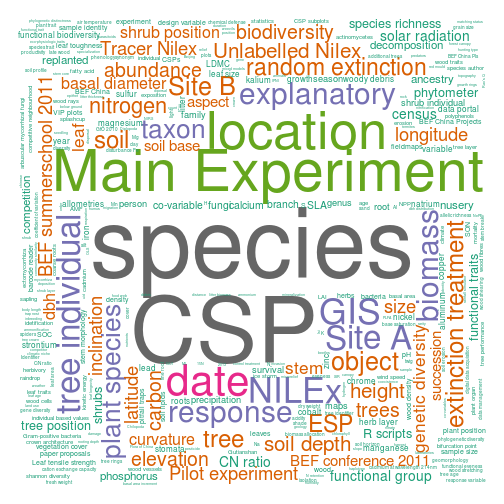
\includegraphics{figure/vizalize_keywords.png}
\caption{plot of chunk vizalize\_keywords}
\end{figure}

\subsubsection{Tables}

\end{document}
